
\section{Experimental Details}

\subsection{Training Settings}
\label{app:training_details}

We conduct three main experiments to study these phenomena.
The JustRL and DeepScaleR settings share the same student initialization and training data, while the Qwen3-4B
setting uses a base Qwen3 student and OpenThoughts3 prompts. The differences between the settings are summarized in Table~\ref{tab:appendix_training_protocol}.

\begin{center}
    \centering
    \small
    \setlength{\tabcolsep}{2.5pt}
    \captionof{table}{\textbf{Training settings used in the main experiments.}
    The teacher is fixed throughout OPD training.}
    \label{tab:appendix_training_protocol}
    \begin{tabular}{@{}lp{0.215\textwidth}p{0.235\textwidth}p{0.195\textwidth}cc@{}}
        \toprule
        Setting & Teacher & Student initialization & Training data & Length limit & LR \\
        \midrule
        JustRL & JustRL-1.5B
        & DeepSeek-R1-Distill-Qwen-1.5B
        & DeepMath-103K, level $\geq 6$ & 16,384 & $10^{-5}$ \\
        DeepScaleR & DeepScaleR-1.5B-Preview
        & DeepSeek-R1-Distill-Qwen-1.5B
        & DeepMath-103K, level $\geq 6$ & 16,384 & $10^{-5}$ \\
        Qwen3-4B & Qwen3-4B
        & Qwen3-1.7B-Base
        & OpenThoughts3 OPD 30K & 8,192 & $10^{-5}$ \\
        \bottomrule
    \end{tabular}
\end{center}

Each setting runs for 100 rollout iterations.
At each iteration, the student samples 8 responses for each of 32 prompts at
temperature $1.0$ and top-$p$ $1.0$, producing 256 responses and two optimizer
updates with global batch size 128. We use Adam with $\beta_1=0.9$,
$\beta_2=0.98$, weight decay $0.1$, no learning-rate warmup, PPO clipping
$\epsilon=0.2$, and an approximate reference-KL coefficient of $0.001$ toward
the fixed initialization $S_{\mathrm{INIT}}$.

The loss mask covers response tokens only.
Each sample is first averaged over its unmasked response tokens, and the resulting
values are then averaged over the global batch, so that long and short responses
contribute equally.
All runs use eight NVIDIA H100 GPUs.
Checkpoints are named by rollout count: the
initialization $S_{\mathrm{INIT}}$ together with iterations 20, 40, 60, 80, and
100, where iteration 100 gives $S_{\mathrm{OPD}}$.

\subsection{DeepScaleR Teacher-Temperature Pilot}
\label{app:deepscaler_temperature_pilot}

We ran two small temperature studies before fixing the DeepScaleR setting.
First, Table~\ref{tab:deepscaler_teacher_temperature} evaluates the frozen
DeepScaleR-1.5B-Preview teacher itself. For every temperature, we draw one
response per problem at top-$p$ $1.0$ with an 8,192-token limit and score it
with the verl verifier. The macro average weights AMC23, AIME24, and AIME25
equally despite their different problem counts.

\begin{center}
    \centering
    \small
    \setlength{\tabcolsep}{5.0pt}
    \captionof{table}{\textbf{Standalone teacher accuracy depends on the generation-sampling temperature.}
    Accuracy is in percent; Macro gives equal weight to the three benchmarks, and bold marks each column maximum.}
    \label{tab:deepscaler_teacher_temperature}
    \begin{tabular}{@{}lrrrr@{}}
        \toprule
        Temperature & AMC23 & AIME24 & AIME25 & Macro \\
        \midrule
        0.1 & 66.27 & 23.33 & \textbf{30.00} & 39.87 \\
        0.5 & \textbf{67.47} & 30.00 & 26.67 & 41.38 \\
        0.75 & 65.06 & \textbf{36.67} & 23.33 & \textbf{41.69} \\
        1 & 56.63 & 20.00 & 10.00 & 28.88 \\
        1.5 & 0.00 & 0.00 & 0.00 & 0.00 \\
        \bottomrule
    \end{tabular}
\end{center}


The training pilot in Figure~\ref{fig:deepscaler_temperature_pilot} instead
varies the temperature applied to the teacher logits when scoring student
rollouts. Each temperature corresponds to one training run. At each displayed
checkpoint, we evaluate the student with four responses per problem sampled at
temperature $1.0$, top-$p$ $1.0$, and a 16,384-token limit; we average within
each problem and then give the three benchmarks equal weight. The $T=1.5$ run
has observations only through iteration 20.

\begin{figure}[t]
    \centering
    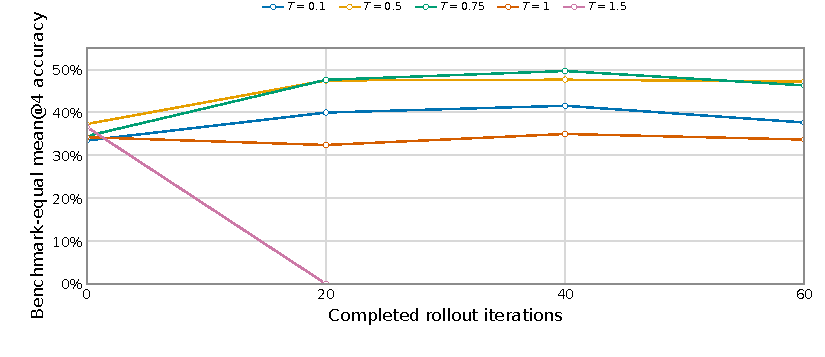
\includegraphics[width=\textwidth]{figures/appendix/deepscaler_temperature_pilot.pdf}
    \caption{
        \textbf{Intermediate teacher-scoring temperatures give the strongest
        single-run student trajectories in the pilot.}
        Benchmark-equal student mean@4 accuracy is plotted against completed
        rollout iterations for the five teacher-scoring temperatures.
    }
    \label{fig:deepscaler_temperature_pilot}
\end{figure}
\FloatBarrier

These pilots support only a working choice, not an optimum. In the standalone
teacher study, $T=0.75$ has macro accuracy $41.69\%$, just $0.31$ percentage
points above $T=0.5$; weighting all 143 problems equally reverses the ordering
($50.35\%$ versus $51.05\%$). The teacher study uses one sample per problem,
and every training curve is a single run with unequal coverage at $T=1.5$.
Together with the strongest observed training point at $T=0.75$, these results
motivated adopting $0.75$ as the working temperature, but do not establish
that it is optimal.

\subsection{Evaluation Protocol}
\label{app:eval_protocol}

We use two evaluation protocols, and they differ only in how many responses are
drawn per problem. Both sample at top-$p$ $1.0$, use the same generation length
limit as training, and serialize prompts with the template described in
Appendix~\ref{app:prompts}. The sampling temperature follows the model being
evaluated rather than the protocol. In the JustRL setting and the DeepScaleR setting, $S_{\mathrm{INIT}}$
and $S_{\mathrm{OPD}}$ are both sampled at $T=1.0$, matching the rollout
temperature used in training.

\paragraph{Routine evaluation.}
Endpoint and per-checkpoint accuracies are reported as mean@4: we draw four
responses per problem, and calculate average accuracy among all the responses. This protocol is
used for the accuracy columns in Section~\ref{sec:5_2} and for the accuracy
traces over training.

\paragraph{Large-pool evaluation.}
The coverage and \passk{k} analyses in Section~\ref{sec:opd_phenomena} require a
much larger budget. For each model and each of the 90 AIME24--26 problems we
draw $n=256$ responses. This pool supports \passk{k} for
$k\in\{1,2,4,8,16,32,64,128,256\}$ and the per-problem success rate
$\hat p_m(q)$, defined as the fraction of verifier-correct responses among the
256 samples.

\paragraph{Conditional extension for the coverage audit.}
For the audit in Appendix~\ref{app:coverage_records} we extend sampling only
where it can change the conclusion. For every problem covered by
$S_{\mathrm{OPD}}$ but not by $S_{\mathrm{INIT}}$ at $n=256$, we draw a further
768 responses from $S_{\mathrm{INIT}}$, giving a conditional pool of 1{,}024
responses for that problem. The prompt, temperature, top-$p$, and length limit
are unchanged; only the number of samples increases.

\paragraph{The audit protocol is deliberately one-sided.}
Both halves of the audit act in a single direction, and we state this
explicitly rather than leave it to be inferred. The additional sampling is
spent only on problems that $S_{\mathrm{OPD}}$ covers and $S_{\mathrm{INIT}}$
does not; the reverse case---covered by $S_{\mathrm{INIT}}$ but not by
$S_{\mathrm{OPD}}$---never receives a larger $S_{\mathrm{OPD}}$ pool. Manual
review is applied to the same candidate list, where it reinstates verifier
misses among $S_{\mathrm{INIT}}$ responses and rejects invalid
$S_{\mathrm{OPD}}$ derivations. Relative to the unaudited 256-response pools,
the procedure can therefore only raise $S_{\mathrm{INIT}}$ coverage and only
lower $S_{\mathrm{OPD}}$ coverage, which is the direction that favors the
conclusion of Section~\ref{sec:opd_phenomena}.

We chose this design because a symmetric audit at equal budget would spend most
of it on problems whose status is not in question, and because the claim under
test is one-sided: a single surviving $S_{\mathrm{OPD}}$-only problem would
refute it, whereas additional $S_{\mathrm{INIT}}$-only problems would not
change it. The cost is that the audited partition in
Table~\ref{tab:appendix_coverage_sets} is not a symmetric measurement of the
two models. It should be read as an upper bound on $S_{\mathrm{INIT}}$
coverage and a lower bound on $S_{\mathrm{OPD}}$ coverage under this protocol,
so the empty $S_{\mathrm{OPD}}$-only column reports that no candidate survived
a search directed against it, not that the two supports were compared on equal
terms. The audited $S_{\mathrm{INIT}}$ and $S_{\mathrm{OPD}}$ totals are
therefore not on the same footing, and their difference overstates the true
gap.

A second consequence is that the candidate list differs between the two teacher
settings, so the two rows of Table~\ref{tab:appendix_coverage_sets} audit the
same $S_{\mathrm{INIT}}$ checkpoint under different budgets. We resolve this by
reporting a single $S_{\mathrm{INIT}}$ set: the union of the problems it is
found to solve under either audit. This is sound because $S_{\mathrm{INIT}}$ is
one checkpoint drawing on one shared pool of 256 responses per problem, so a
solution recovered in one audit is evidence about the checkpoint and not about
the teacher it was audited alongside. No counterpart exists on the
$S_{\mathrm{OPD}}$ side, where the two rows are different models. Pooling in
this way gives $S_{\mathrm{INIT}}$ the combined budget of both audits and so
widens the asymmetry above; it cannot create an $S_{\mathrm{OPD}}$-only
problem, since enlarging $S_{\mathrm{INIT}}$ can only remove entries from that
column.


\paragraph{Estimating \passk{k}.}
Reporting \passk{k} from a single group of $k$ responses is high variance. For a
problem with $c$ correct responses among $n$, we instead use the standard
unbiased estimator of the probability that a group of $k$ responses drawn
without replacement from the pool contains at least one correct response
\citep{chen2021evaluating},
\begin{equation}
    \passk{k}
    =
    \mathbb{E}_{q}
    \left[
        1-\frac{\binom{n-c_q}{k}}{\binom{n}{k}}
    \right],
    \label{eq:pass_at_k}
\end{equation}
evaluated at $n=256$ and averaged over problems with equal weight. We compute
the ratio as $\prod_{i=0}^{k-1}(n-c_q-i)/(n-i)$ to avoid large binomial
coefficients. At $k=n$ the estimator reduces to an indicator of whether the pool
contains any correct response, so \passk{256} equals the observed coverage of
that pool.

\paragraph{Correctness.}
Correctness is always recomputed from the response text; we do not reuse the
reward labels stored during rollout, which are produced by a different scorer
and under a different generation setting. All three benchmarks have
non-negative integer answers, and the verifier extracts a predicted integer with
the first rule that applies: the content of the last \verb|\boxed{...}| holding
an integer; otherwise the last integer introduced by an explicit answer cue such
as \texttt{final answer is}; otherwise the response as a whole, if it consists
of a single integer. A response with no extractable integer counts as incorrect.
Prediction and reference are compared after integer normalization, so the
verifier accepts no symbolic equivalence beyond leading-zero and whitespace
differences.

The second and third rules make the verifier permissive: a response can be
scored correct without ever emitting a boxed answer. This matters for the
coverage audit, where accepting an accidental hit from $S_{\mathrm{INIT}}$ would
weaken the claim it supports. We therefore inspect every
$S_{\mathrm{INIT}}$ recovery found in the extended pools by hand rather than
trusting the verifier alone, and report the outcome per problem in
Appendix~\ref{app:coverage_records}.

\subsection{Prompt Templates}
\label{app:prompts}

Training and evaluation examples contain one user message and no system
message. Each training example already includes the instruction
\texttt{\detokenize{Please reason step by step, and put your final answer within \boxed{}.}}
after the problem statement, separated by a newline in DeepMath and a space
in OpenThoughts3. We include the same instruction for mathematics evaluation
and serialize the message with the student's chat template. Routine
evaluation uses the same template as training. Below, \texttt{\{QUESTION\}}
denotes the problem statement without this instruction.

\paragraph{JustRL and DeepScaleR settings.}
Both use the DeepSeek-R1-Distill-Qwen-1.5B student template:
\begingroup
\expandafter\def\csname u8:｜\endcsname{\textbar}
\expandafter\def\csname u8:▁\endcsname{\rule{0.5em}{0.4pt}}
\begin{promptbox}{JustRL / DeepScaleR Prompt \textbar\ DeepSeek-R1-Distill-Qwen-1.5B}
\fontsize{7}{9}\selectfont
\begin{verbatim}
<｜begin▁of▁sentence｜><｜User｜>{QUESTION}
Please reason step by step, and put your final answer within \boxed{}.<｜Assistant｜><think>
\end{verbatim}
\end{promptbox}
\endgroup
The assistant prefix ends with \texttt{<think>} followed by a newline,
leaving the reasoning block open for generation.

\begin{samepage}
\paragraph{Qwen3-4B setting.}
We use the Qwen3-1.7B student template with thinking mode disabled.
Specifically, we prefill the assistant turn with an empty reasoning block,
\texttt{<think>} followed by two newlines, \texttt{</think>}, and two more
newlines. Generation therefore starts after the closed block. The serialized
prompt is:
\begin{promptbox}{Qwen3-4B Setting Prompt \textbar\ Qwen3-1.7B \textbar\ Thinking Disabled}
\fontsize{7}{9}\selectfont
\begin{verbatim}
<|im_start|>user
{QUESTION} Please reason step by step, and put your final answer within \boxed{}.<|im_end|>
<|im_start|>assistant
<think>

</think>

\end{verbatim}
\end{promptbox}
Disabling thinking mode changes this assistant prefix; the user instruction
to reason step by step remains in the prompt.
\end{samepage}

\paragraph{Teacher scoring.}
After the student generates a response, we feed the full token sequence---the
serialized prompt and the student-generated response---into the teacher in a
single forward pass to obtain the next-token distributions at the response
positions for distillation. The teacher generates no new tokens
(\texttt{max\_new\_tokens=0}). We use the student's original token sequence
directly, without reapplying a chat template or adding any instructions.

\FloatBarrier

\section{Observed Solvable Sets}
\label{app:coverage_records}

We first construct candidate solvable sets from problems with at least one
verifier-correct response in the original 256-response pools. We then refine
these sets through targeted sampling and manual review: invalid derivations
are excluded, and valid solutions missed by the automatic verifier are
reinstated. Table~\ref{tab:appendix_coverage_sets} reports the resulting
audited partition of all 90 AIME24--26 problems under each teacher.
The four columns form a disjoint partition: covered by both
$S_{\mathrm{INIT}}$ and $S_{\mathrm{OPD}}$, covered only by one of them, or
covered by neither. Problem numbers are listed explicitly within each dataset.

The audit combines additional sampling with review of the existing outputs.
We take every problem that is covered
by $S_{\mathrm{OPD}}$ but not by $S_{\mathrm{INIT}}$ among 256 responses and
extend the $S_{\mathrm{INIT}}$ pool to 1,024 responses. This recovers seven
cases: JustRL AIME25-025 and AIME26-010, and DeepScaleR AIME25-014,
AIME25-023, AIME25-025, AIME26-010, and AIME26-022. Manual review also checks the validity of
$S_{\mathrm{OPD}}$ derivations among the candidate problems, including cases
already recovered by additional sampling. The JustRL AIME25-020 and
DeepScaleR AIME25-014 and AIME25-025 derivations are invalid despite reaching
the correct final answer. The latter two problems are therefore assigned to
the $S_{\mathrm{INIT}}$-only set.

For JustRL AIME26-022 and AIME26-027, the automatic verifier records no
$S_{\mathrm{INIT}}$ hit in the 1,024-response pools. Manual review identifies
valid $S_{\mathrm{INIT}}$ solutions in the existing outputs and corrects these
verifier misses; it does not use a separate batch of generations. These cases
are assigned to the shared set.
Table~\ref{tab:appendix_coverage_audit} distinguishes recoveries by additional
sampling from corrections to automatic verification.

\begin{center}
\captionof{table}{\textbf{Audited observed-solvable-set partitions.}
Each cell gives the number of problems followed by their three-digit suffixes.}
\label{tab:appendix_coverage_sets}
\centering
\scriptsize
\setlength{\tabcolsep}{2.2pt}
\begin{tabular}{llp{0.31\textwidth}p{0.12\textwidth}p{0.10\textwidth}p{0.20\textwidth}}
\toprule
Teacher & Data & Both & $S_{\mathrm{INIT}}$ only & $S_{\mathrm{OPD}}$ only & Neither \\
\midrule
JustRL & AIME24
& \textbf{24}: 001--007, 009, 010, 013--022, 025--029
& \textbf{1}: 023 & \textbf{0}: --
& \textbf{5}: 008, 011, 012, 024, 030 \\
JustRL & AIME25
& \textbf{18}: 001--006, 008, 009, 012, 016, 017, 019, 021, 022, 024, 025, 027, 029
& \textbf{6}: 010, 013, 014, 023, 028, 030 & \textbf{0}: --
& \textbf{6}: 007, 011, 015, 018, 020, 026 \\
JustRL & AIME26
& \textbf{23}: 001--008, 010, 012--014, 016, 018--027
& \textbf{1}: 011 & \textbf{0}: --
& \textbf{6}: 009, 015, 017, 028--030 \\
\midrule
DeepScaleR & AIME24
& \textbf{23}: 001--007, 009, 010, 013--022, 025--028
& \textbf{2}: 023, 029 & \textbf{0}: --
& \textbf{5}: 008, 011, 012, 024, 030 \\
DeepScaleR & AIME25
& \textbf{18}: 001--006, 008, 009, 012, 016, 017, 019, 021--024, 027, 029
& \textbf{6}: 010, 013, 014, 025, 028, 030 & \textbf{0}: --
& \textbf{6}: 007, 011, 015, 018, 020, 026 \\
DeepScaleR & AIME26
& \textbf{22}: 001--008, 010, 012--014, 016, 018--026
& \textbf{2}: 011, 027 & \textbf{0}: --
& \textbf{6}: 009, 015, 017, 028--030 \\
\bottomrule
\end{tabular}
\end{center}

\begin{center}
\captionof{table}{\textbf{Resolution of the raw $S_{\mathrm{OPD}}$-only cases.}
The third column records how a correct $S_{\mathrm{INIT}}$ response was
obtained. ``Extended sampling'' means the verifier accepted a response drawn
while extending the pool to 1,024. ``Manual review'' means a correct response
was already present and had been missed by the verifier, so no additional
generation was needed. ``None'' means neither route produced one.}
\label{tab:appendix_coverage_audit}
\centering
\small
\setlength{\tabcolsep}{3.5pt}
\begin{tabular}{@{}llp{0.22\textwidth}p{0.17\textwidth}p{0.27\textwidth}@{}}
\toprule
Teacher & Problem & $S_{\mathrm{INIT}}$ solution found by & $S_{\mathrm{OPD}}$ derivation & Resolution \\
\midrule
JustRL & AIME25-020 & None & Invalid & Removed as an accidental verifier hit \\
JustRL & AIME25-025 & Extended sampling & Valid & Shared \\
JustRL & AIME26-010 & Extended sampling & Valid & Shared \\
JustRL & AIME26-022 & Manual review & Valid & Shared \\
JustRL & AIME26-027 & Manual review & Valid & Shared \\
\midrule
DeepScaleR & AIME25-014 & Extended sampling & Invalid & $S_{\mathrm{INIT}}$ only \\
DeepScaleR & AIME25-023 & Extended sampling & Valid & Shared \\
DeepScaleR & AIME25-025 & Extended sampling & Invalid & $S_{\mathrm{INIT}}$ only \\
DeepScaleR & AIME26-010 & Extended sampling & Not needed & Shared \\
DeepScaleR & AIME26-022 & Extended sampling & Valid (two reviews) & Shared \\
\bottomrule
\end{tabular}
\end{center}


These sets describe the responses observed under the stated sampling and
manual-audit protocol. They do not establish equality of model support or
zero probability for any response under $S_{\mathrm{INIT}}$.

\FloatBarrier

\section{Min-10NN Distance}
\label{app:response_geometry}

Min-10NN measures how tightly responses to the same problem concentrate in
surface form. For two decoded responses $a$ and $b$, we use character-level
normalized Levenshtein distance
\begin{equation}
    d(a,b)=
    \begin{cases}
        0, & |a|=|b|=0,\\
        \operatorname{Lev}(a,b)/\max\{|a|,|b|\}, & \text{otherwise}.
    \end{cases}
\end{equation}

Let $R=\{r_i\}_{i=1}^{16}$ be 16 responses to one problem. For each response,
we compute its distance to the nearest other response,
\begin{equation}
    \delta_i=\min_{j\ne i}d(r_i,r_j).
\end{equation}
After sorting these values as
$\delta_{(1)}\leq\cdots\leq\delta_{(16)}$, Min-10NN is
\begin{equation}
    \operatorname{Min\text{-}10NN}(R)
    =\frac{1}{10}\sum_{i=1}^{10}\delta_{(i)}.
\end{equation}
A smaller value means that the ten most tightly clustered responses are more
similar. When 32 responses are available, we sample 16 without replacement,
average Min-10NN over 100 repetitions, and then average across problems. The
metric captures character-level concentration only; it does not measure
semantic equivalence or response quality.

\FloatBarrier

\section{Response Case Study}
\label{app:response_excerpts}

Figure~\ref{fig:qualitative_response_examples} gives the examples of the
excerpts condensed in Figure~\ref{fig:main_teaser}b. All four responses come
from the Qwen3-4B setting before any OPD update: (a) is a free generation of
the teacher, and (b)--(d) are sampled from $S_{\mathrm{INIT}}$, with (c) and
(d) drawn from the responses the teacher ranks as most preferred under the
decile partition of Section~\ref{sec:teacher_selection}.

\begin{figure*}[t]
    \centering
    \begingroup
    \definecolor{responsehealthyframe}{HTML}{3C7D73}
    \definecolor{responsehealthyfill}{HTML}{F1F8F6}
    \definecolor{responsecollapseframe}{HTML}{B85245}
    \definecolor{responsecollapsefill}{HTML}{FCF3F1}
    \setlength{\fboxsep}{5pt}
    \setlength{\fboxrule}{0.55pt}
    \newcommand{\responseexample}[5]{%
        \begin{minipage}[t]{0.485\textwidth}
            \fcolorbox{#1}{#2}{%
                \parbox[t][25mm][t]{\dimexpr\linewidth-2\fboxsep-2\fboxrule\relax}{%
                    \raggedright
                    \scriptsize
                    \textbf{#3}\par
                    {\fontsize{6.8}{7.5}\selectfont\textbf{#4}}\par
                    \vspace{1.5pt}
                    #5
                }%
            }
        \end{minipage}%
    }

    \responseexample{responsehealthyframe}{responsehealthyfill}
        {(a) Teacher: coherent solution}{correct; 842 tokens}{%
        ``Number of \textbf{grand prize} outcomes: 1. \ldots\ Number of
        \textbf{prize} outcomes ($\geq 2$ matches): 115. \ldots
        $P(\text{Grand Prize}\mid\text{Prize})=1/115$.
        Thus, $m+n=1+115=116$.''}
    \hfill
    \responseexample{responsehealthyframe}{responsehealthyfill}
        {(b) $S_{\mathrm{INIT}}$: coherent solution}{correct; 771 tokens}{%
        ``Jen has exactly 2 of the chosen 4 numbers:
        $C(4,2)C(6,2)=90$. \ldots\ Exactly 3: 24; all 4: 1.
        So, the total number of ways to win a prize is
        $90+24+1=115$. \ldots
        $P(\text{grand prize}\mid\text{prize})=1/115$.
        \ldots\ \fbox{116}.''}

    \vspace{4pt}

    \responseexample{responsecollapseframe}{responsecollapsefill}
        {(c) $S_{\mathrm{INIT}}$, teacher-preferred: repeated reconsideration}{incorrect; 7,311 tokens}{%
        ``$17{,}499{,}840/661{,}680=26.5$.
        \textbf{Wait, this is incorrect.} The calculation is not correct.
        Instead, we should compute the number of valid sequences. Let's go
        back. \ldots\ But this is not correct. \textbf{Wait, for the last word}
        to be GY, \ldots\ \textbf{Wait, this is not correct.}''}
    \hfill
    \responseexample{responsecollapseframe}{responsecollapsefill}
        {(d) $S_{\mathrm{INIT}}$, teacher-preferred: mechanical repetition}{correct; 8,192 tokens; truncated}{%
        ``\textbf{Final Answer: \fbox{116}} \ldots\
        \textbf{Answer: \fbox{116}} \ldots\
        \textbf{Final Answer: \fbox{116}} \ldots\
        \textbf{Answer: \fbox{116}} \ldots''\par
        \vspace{2pt}
        The same answer line repeats 365 times until the generation length
        limit.}
    \endgroup
    \caption{
        \textbf{Illustrative response excerpts from the Qwen3-4B setting.}
        The teacher and a typical $S_{\mathrm{INIT}}$ response give coherent
        solutions, whereas the $S_{\mathrm{INIT}}$ responses the teacher most
        prefers repeatedly restart their reasoning or mechanically repeat an
        answer until the generation length limit. All four excerpts predate any
        OPD update. Ellipses mark omitted text. These examples illustrate
        behaviors and do not estimate their prevalence.
    }
    \label{fig:qualitative_response_examples}
\end{figure*}


\FloatBarrier

\section{High-Advantage Responses from the Initial Student}
\label{app:high_advantage_examples}

We present three responses sampled from Qwen3-1.7B-Base before any OPD
update and scored by the Qwen3-4B teacher. All three belong to the
highest-advantage group, A10, in the analysis of
Section~\ref{sec:teacher_selection} and illustrate excessive length and
mechanical repetition already present under $S_{\mathrm{INIT}}$.
All three are incorrect and contain no parseable final answer.

\paragraph{Reading the complete responses.}
Each response consists almost entirely of a repeated string. We specify its
complete content using exact repetition counts: $+$ denotes concatenation
without an added separator, and $\operatorname{repeat}(s,n)$ denotes $n$
consecutive copies of $s$. Quotation marks delimit strings and are not part
of the response; \texttt{\textbackslash n} denotes a newline. Unicode
characters are written as \texttt{\textbackslash uXXXX} escapes. No text is
omitted from these representations. Prompt mathematics below is
typeset for readability. Every prompt ends with: ``Please reason step by
step, and put your final answer within \texttt{\textbackslash boxed\{\}}.''

\subsection{Length-Cap Repetition}

\paragraph{Prompt (AIME24, \texttt{aime24\_001}).}
Every morning Aya goes for a $9$-kilometer-long walk and stops at a coffee
shop afterwards. When she walks at a constant speed of $s$ kilometers per
hour, the walk takes her 4 hours, including $t$ minutes spent in the coffee
shop. When she walks $s+2$ kilometers per hour, the walk takes her 2 hours
and 24 minutes, including $t$ minutes spent in the coffee shop. Suppose Aya
walks at $s+\frac{1}{2}$ kilometers per hour. Find the number of minutes the
walk takes her, including the $t$ minutes spent in the coffee shop.

\paragraph{Response (sample 65).}
\begin{quote}
\small\ttfamily
"\textbackslash uFFFD\textbackslash uFFFD\textbackslash u6001\ T 10T 50 10 1 10 10"\\
\normalfont $+\;\operatorname{repeat}($\texttt{"T 10"}$,\;2043)$
\end{quote}
The response mechanically repeats \texttt{T 10} until it reaches the
8,192-token generation cap. The two initial
\texttt{\textbackslash uFFFD} characters are present in the stored response.

\subsection{Severe Repetition without Reaching the Length Cap}

\paragraph{Prompt (AIME25, \texttt{aime25\_028}).}
Let the sequence of rationals $x_1,x_2,\ldots$ be defined such that
$x_1=\frac{25}{11}$ and
$x_{k+1}=\frac{1}{3}\left(x_k+\frac{1}{x_k}-1\right)$.
$x_{2025}$ can be expressed as $\frac{m}{n}$ for relatively prime positive
integers $m$ and $n$. Find the remainder when $m+n$ is divided by 1000.

\paragraph{Response (sample 110).}
\begin{quote}
\small
$\operatorname{repeat}($\texttt{".slfwith\textbackslash n"}$,\;2154)
+$ \texttt{".slfwith"}
\end{quote}
The response consists of repeated \texttt{.slfwith} lines and ends after
6,465 recorded tokens, showing that severe repetition can occur without
reaching the generation cap.

\subsection{Severe Repetition at the Length Cap}

\paragraph{Prompt (AIME25, \texttt{aime25\_013}).}
Alex divides a disk into four quadrants with two perpendicular diameters
intersecting at the center of the disk. He draws 25 more line segments
through the disk, drawing each segment by selecting two points at random
on the perimeter of the disk in different quadrants and connecting those
two points. Find the expected number of regions into which these 27 line
segments divide the disk.

\paragraph{Response (sample 58).}
\begin{quote}
\small\ttfamily
"\textbackslash u6CD5\ newVal89\textbackslash u6CD5\ newVal8\textbackslash u6CD5\ newVal8"\\
\normalfont $+\;\operatorname{repeat}($\texttt{"\textbackslash u6CD5\ newVal"}$,\;4091)$
\end{quote}
The response repeats the same fragment until it reaches the 8,192-token
generation cap, exhibiting both excessive length and severe repetition.

Together, these cases illustrate how excessively long and repetitive responses can receive
high relative teacher advantage already under $S_{\mathrm{INIT}}$.


\FloatBarrier

\section{Training Details for the Candidate-Pool Interventions}
\label{app:intervention_details}

Section~\ref{sec:5_2} compares three Qwen3-4B teacher settings. The baseline
and masked settings initialize the student from Qwen3-1.7B-Base. The warmup
setting instead initializes it from the Qwen3-1.7B-SFT checkpoint released by
\citet{li2026rethinkingopd} and uses that model as the fixed reference.
All three use OpenThoughts3 prompts, temperature $1.0$, an
8,192-token generation length limit, and the optimization settings in
Appendix~\ref{app:training_details}.

\paragraph{Loss masking for truncated or failed responses.}
The baseline trains on all sampled responses, including those that reach the
generation length limit. In the masked setting, we set the loss mask to zero
for truncated or failed responses; completed responses retain nonzero loss
masks and contribute to training. Truncated or failed responses remain in reward and
advantage normalization but contribute no policy, reference-KL, or entropy
gradient. The loss is first averaged over unmasked response tokens within
each sample and then over samples in the global batch.


\paragraph{Initialization from a released SFT checkpoint.}
The warmup setting directly loads the Qwen3-1.7B-SFT checkpoint released by
\citet{li2026rethinkingopd}; we do not perform an additional SFT stage ourselves.
It changes only the student initialization and fixed reference
from Qwen3-1.7B-Base to Qwen3-1.7B-SFT; the teacher, data, optimizer, sampling
protocol, and evaluation schedule remain fixed. Its higher initial accuracy
is part of the intervention: it tests whether supplying a better initial
candidate pool changes what OPD can amplify.

\FloatBarrier
